\documentclass{classrep}
\usepackage[utf8]{inputenc}
\usepackage{hyperref}
\usepackage{graphicx}
\graphicspath{ {./} }
\usepackage{color}

\studycycle{Informatyka, studia dzienne, I st.}
\coursesemester{VI}

\coursename{Komputerowe systemy rozpoznawania}
\courseyear{2018/2019}

\courseteacher{dr inż. Marcin Kacprowicz}
\coursegroup{Wtorek, 16:15}

\author{
  \studentinfo{Paweł Młynarczyk}{210278} \and
  \studentinfo{Mateusz Kuźniarek}{210245}
}

\title{Zadanie 1 - Ekstrakcja cech, miary podobieństwa, klasyfikacja.}

\begin{document}
\maketitle

\section{Cel}
Celem zadania było zaprojektowanie i implementacja narzędzia, pozwalającego na klasyfikację tekstów przy użyciu algorytmu KNN. Podczas realizacji ćwiczenia, należało zbadać wpływ parametrów takich, jak sposób ekstrakcji cech, czy użyta miara podobieństwa na skuteczność i szybkość procesu klasyfikacji.

\section{Wprowadzenie}
\subsection{Ekstrakcja cech}
W celu szybkiego i efektywnego porównywania tekstów przydatna okazuje się ich reprezentacja w postaci wektora liczb. Współrzędne takiego wektora odpowiadają poszczególnym cechom, opisującym reprezentowany tekst. Proces analizy tekstu i określenia wartości liczbowej dla danej jego własności nazywamy ekstrakcją cech. Wybór odpowiedniego sposobu ekstrakcji jest kluczowy dla efektywnego działania programu. W ramach zadania zaimplementowano 3 takie sposoby.

\subsubsection{TF (Term Frequency)}
Dla każdego słowa kluczowego obliczana jest jego częstotliwość przy pomocy wzoru: 
\begin{equation}
tf(t,d) =  \frac{f_{t,d}}{|d|} \cite{TF_TF-IDF}
\end{equation}
gdzie \(f_{t,d}\) jest liczbą wsytąpień słowa \(t\) w tekście \(d\), a \(|d|\) jest liczbą wszystkich słów w tym tekście. Wartości funkcji \(tf(t,d)\) dla każdego słowa kluczowego stanową współrzędne wektora, reprezentującego dany dokument.

\subsubsection{TF-IDF (term frequency–inverse document frequency)}
Ten sposób ekstrakcji cech wykorzystuje TF(Term Frequency) i wzbogaca je o informację na temat tego, jak często dane słowo znajduje się w dokementach innych niż analizowany. Wartość TF-IDF można uzyskać przy pomocy wzoru: 
\begin{equation}
tfidf(t,d,D) = tf(t,d) \cdot idf(t,D) \cite{TF_TF-IDF}
\end{equation}
gdzie \(tf(t,d)\), jest wartością TF obliczoną przy pomocy woru 1., a \(idf(t,D)\) wyraża się wzorem
\begin{equation}
idf(t,D) = log\frac{|D|}{n} \cite{TF_TF-IDF}
\end{equation}
gdzie \(|D|\) to liczba wszystkich tekstów w analizowanym zbiorze, a \(n\) to liczba tekstów, w których przynajmniej raz znajduje się słowo \(t\).

\subsubsection{Własna metoda ekstrakcji cech}
Trzecim wykorzystanym sposobem była własna metoda ekstrakcji wektora cech. Składała się ona z następujących własności:
\begin{itemize}
	\item Suma wartości TF dla grupy słów kluczowych
	\item Suma wartości podobieństwa słowa kluczowego do analizowanego tekstu przy użyciu miary trigramów. \cite{ANiewSkrypt}
	\item Długość tekstu
	\item Średnia z występujących w tekście liczb
	\item Średnia długość słowa wśród 4 najdłuższych słów
\end{itemize}


\subsection{Normalizacja}
Otrzymane na powyższe sposoby cechy zostały następnie znormalizowane przy użyciu wzoru:
\begin{equation}
x' = \frac{x-x_{min}}{x_{max}-x_{min}} \cite{MLWiki}
\end{equation}

\subsection{Algorytm KNN}
Do klasyfikacji tekstów wykorzystany został algorytm KNN(k-nearest neighbors). Pozwala on na przypisanie danej próbce klasy na podstawie tego, jak zaklsyfikowani są jej najbliżsi sąsiedzi. Bliskość dwóch próbek zdefiniowana jest za pomocą odpowiedniej metryki lub miary podobieństwa. \cite{KNNWiki}

W ramach zadania zaimplementowano następujące metryki: \newline
Metryka euklidesowa:
\begin{equation}
d(p,q) = \sqrt{\sum_{i=1}^{n} (p_{i} -q_{i})^{2}} \cite{ANiewSkrypt}
\end{equation}
Metryka uliczna:
\begin{equation}
d(p,q) = \sum_{i=1}^{n} |p_{i} -q_{i}| \cite{ANiewSkrypt}
\end{equation}
Metryka Czebyszewa:
\begin{equation}
d(p,q) = max_{i}(p_{i} -q_{i}) \cite{ChebyshevWiki}
\end{equation}
gdzie \(n\) jest długością wektorów \(p = [p_{1}, p_{2}, ..., p_{n}]\) oraz \(q = [q_{1}, q_{2}, ..., q_{n}]\) są wektorami, między którymi liczona jest odległość. 

Oprócz tego zaimplementowano następujące miary podobieństwa: \newline
Minimum-maximum
\begin{equation}
r_{mm}(p,q) = \frac{\sum_{i=1}^{n}min(p_{i},q_{i})}{\sum_{i=1}^{n}max(p_{i},q_{i})} \cite{ANiewSkrypt}
\end{equation}
Średnia arytmetyczna-minimum
\begin{equation}
r_{am}(p,q) = \frac{\sum_{i=1}^{n}min(p_{i},q_{i})}{\frac{1}{2}\sum_{i=1}^{n}(p_{i}+q_{i})} \cite{ANiewSkrypt}
\end{equation}
Własna propozycja miary podobieństwa
\begin{equation}
r_{wm}(p,q) = (r_{mm}(p,q))^{2}
\end{equation}

Powyższych metryk oraz miar podobieństw użyto do znalezieniu k najbliższych analizowanemu tekstowi próbek. Na ich podstawie tekst mógł zostać zaklasyfikowany do najbardziej licznej wśród wybranych sąsiadów z klas. W przypadku wielu jednakowo-licznych klas, wybierano tę, której próbka znajdowała się najbliżej analizowanego tekstu.

\section{Opis implementacji}

W celu realizacji zadania została napisana aplikacja okienkowa w języku Java, natomiast graficzny interfejs użytkownika został wykonany w technologii JavaFX.
W projekcie skorzystano z natępujących bibliotek:
\begin{itemize}
	\item commons-io - bibliteka umożliwiająca deserializację plików xml; \cite{commons-io}
	\item javafx-fxml - biblioteka używana w warstwię prezentacji do reprezentacji graficznego interfejsu użytkownika; \cite{JavaFX}
	\item snowball-stemmer - biblioteka udostępniająca stemmer; \cite{Stemmer}
\end{itemize}

Projekt podzielono na dwa główne pakiety, przechowujący klasy warstwy prezentacji pakiet \textit{gui}, oraz pakiet \textit{logic}, w którym jest zawarta cała logika aplikacji. Na pakiet \textit{logic} składają się liczne podpakiety, które wydzielają poszczególne funkcjonalności aplikacji jeszcze bardziej. Są to: pakiet \textit{classification}, którego klasy realizują zagadnienie klasyfikacji obiektów tekstowych; pakiet \textit{extractors}, który zawiera w sobie ekstraktory cech; pakiet \textit{features} zawierający w sobie klasy, reprezentujące cechy obiektów; pakiet \textit{metrics}, którego klasy realizują poszczególne metryki; oraz pakiet \textit{utils} zawierający w sobie wszystkie klasy wspomagające działanie programu, niezwiązane bezpośrednio z ideą działania sieci knn.

Opis poszczególnych klas w ramach pakietu:

\begin{itemize}
	\item gui
	\begin{itemize}
		\item MainApp.java - klasa uruchomieniowa aplikacji, jej celem jest jedynie skonfigurowanie oraz ustawienie nowej sceny JavaFX;
		\item FXMLController.java - klasa kontrolera JavaFX przypisana do pliku FXML definiująca sposób działania elementów interfejsu użytkownika;
	\end{itemize}
	\item logic.classification
	\begin{itemize}
		\item TextSample.java - klasa reprezentująca próbkę tekstu, będąca reprezentacją badanych artykułów, zawiera informacje o etykiecie, i słowach zawartych w artykule;
		\item ExtractedSample.java - klasa reprezentująca wyekstrahowaną próbkę tekstu, na którą składa się jedynie etykieta oraz wektor cech tej próbki;
		\item Normalizer.java - klasa zdolna normalizować cechy wyekstrahowanej próbki do przedziału [0,1], w oparciu o cechy zbioru obiektów(tu zbioru treningowego);
		\item KNNClasification.java - reprezentacja sieci knn, do najważniejszych metod tej klasy należą metoda \textit{train()}, która bazując na zbiorze testowym, tworzy strukturę sieci, oraz metoda \textit{classify()} dokonująca klasyfikacji obiektów zbioru testowego w oparciu o utworzoną wcześniej strukturę;
	\end{itemize}
	\item logic.extraction
	\begin{itemize}
		\item FeatureExtractor.java - klasa abstrakcyjna ekstraktora cech;
		\item TFExtractor.java - klasa ekstraktora cechy TF;
		\item TFIDFExtractor.java - klasa ekstraktora cech TF-IDF;
		\item CustomExtractor.java - klasa autorskiego ekstraktora cech;
	\end{itemize}
	\item logic.features
	\begin{itemize}
		\item Feature.java - klasa abstrakcyjna cechy;
		\item TermFrequency.java - klasa cechy TF;
		\item TermFrequencyInverseDocumentFrequency.java - klasa cechy TF-IDF; 
		\item CombinedTermFrequency.java - klasa cechy będącej sumą cech TF dla każdego słowa kluczowego;
		\item NGram.java - klasa cechy Ngramów;
		\item CombinedNGram.java - klasa cechy będącej sumą cech NGramów dla każdego słowa kluczowego;
		\item Length.java - klasa cechy długości tekstu;
		\item AverageNumber.java - klasa cechy średniej z liczb występujących w tekście;
		\item LongestWordsAverageLength.java - klasa cechy średniej długości najdłuższych słów występujących w tekście;
	\end{itemize}
	\item logic.metrics
	\begin{itemize}
		\item Metric.java - klasa abstrakcyjna metryki;
		\item EuclideanMetric.java - klasa reprezentacja metrykę Euklidesowską;
		\item ManhattanMetric.java - klasa reprezentacja metrykę Manhattańską (taksówkarską);
		\item ChebyshevMetric.java - klasa reprezentacja metrykę Czebyszewa;
		\item Similarity.java - klasa abstrakcyjna miary podobieństwa;
		\item MinMaxSimilarity.java - klasa reprezentacja miarę podobieństwa Minimum-Maximum;
		\item AverageMinSimilarity.java - klasa reprezentacja miarę podobieństwa Średniej Arytmetycznej-Minimum;
		\item CustomSimilarity.java - klasa reprezentująca własną miarę podobieństwa;
	\end{itemize}
	\item logic.utils
	\begin{itemize}
		\item SgmToXmlConverter.java - klasa konwertera zamieniająca plik sqm, w którym zostały dostarczone dane na plik, xml z którego są potem wczytywane do programu;
		\item ExampleLoader.java - klasa wczytująca teksty z pliku xml i przeprowadzająca wstępną obróbkę tekstu oraz stemizację, celem usprawnienia późniejszego procesu klasyfikacji;
		\item CSVData.java - klasa reprezentująca dane statystyczne zapisywane później do pliku csv;
		\item CSVWriter.java - klasa zapisująca dane powstałe w wyniku klasyfikacji do pliku csv;
	\end{itemize}
\end{itemize}

Podnadto w projekcie znajdują się pliki Scene.fxml oraz Styles.css które opisują elementy graficznego interfejsu użytkownika.

{\color{blue} UML!!!!!!!!!!!!!!!!!!}

\begin{figure}[h]
	\advance\leftskip-4cm
		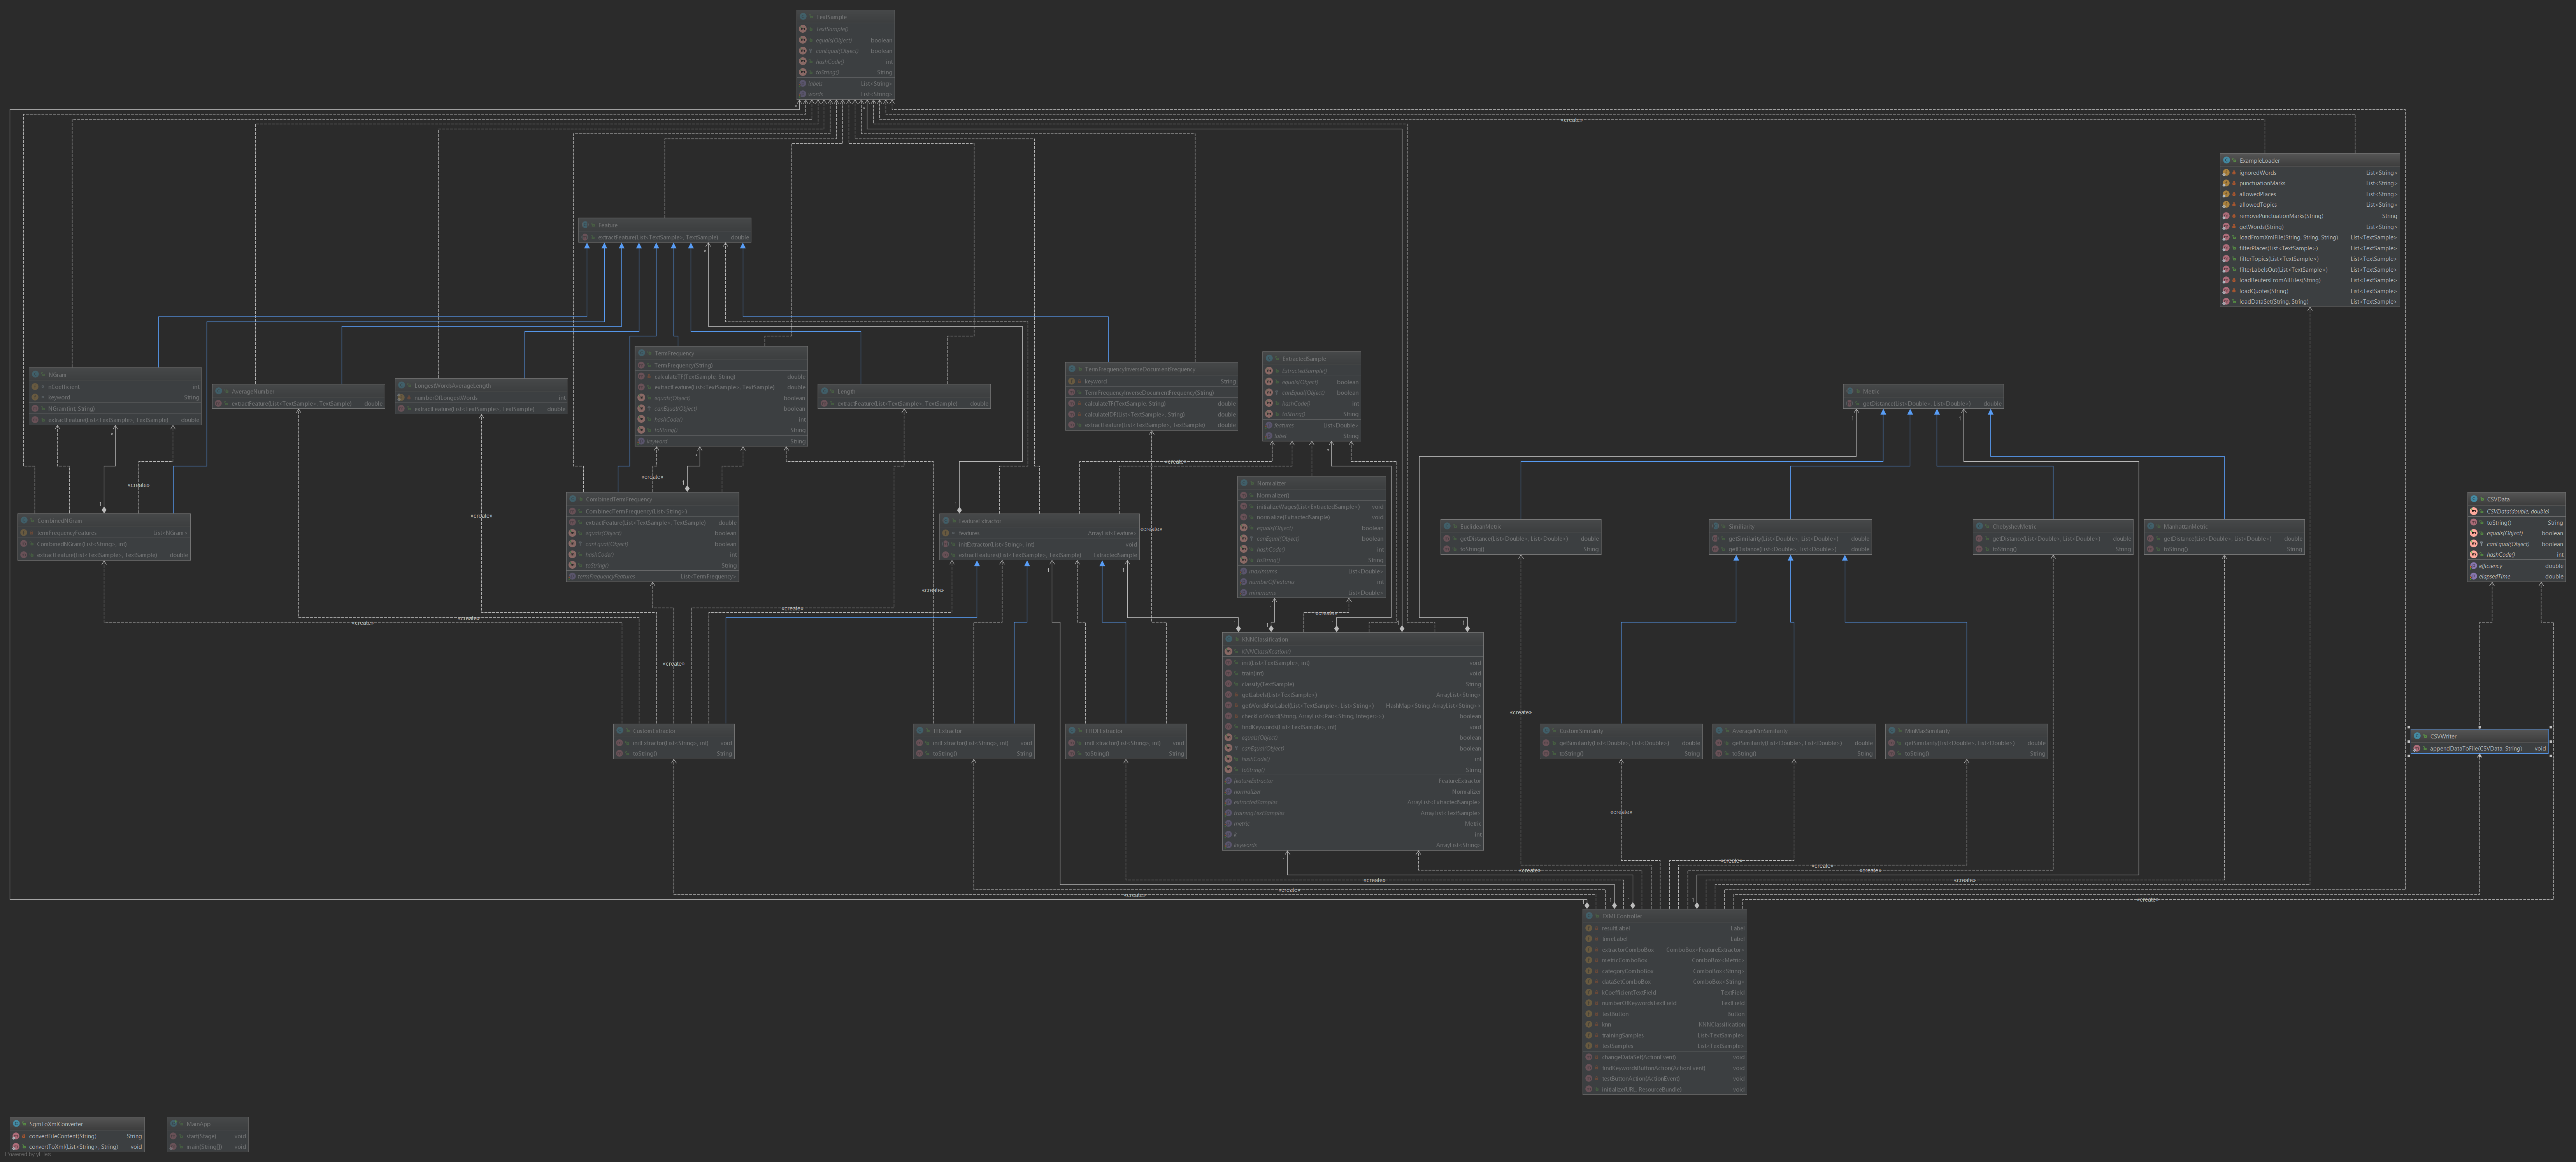
\includegraphics[width=\paperwidth]{ksr_uml}
\end{figure}

\section{Materiały i metody}
Przed rozpoczęciem klasyfikacji analizowane teksty zostały odpowiednio przygotowane do wykorzystania. Treść została podzielona na pojedyncze słowa, które następnie zostały poddane procesowi stemmingu, który to polega na pozbyciu się końcówek fleksyjnych wyrazu. Z tekstu usunięto wszystkie znaki interpunkcyjne, a wielkie litery zamieniono na małe. Następnie, przy pomocy odpowiednio przygotowanej stop-listy, pozbyto się niepożądanych słów, które nie niosły ze sobą większego znaczenia dla procesu klasyfikacji.
We wszystkich, opisanych poniżej eksperymentach słowa kluczowe zostały wyznaczone w ten sam sposób. Z przefiltrowanej listy słów wybrano te, które pojawiały się najczęściej dla danej klasy. 
Do eksperymentów użyto dwóch zbiorów danych. Własnoręcznie opracowany spis cytatów znanych pisarzy oraz dostępny pod \href{http://archive.ics.uci.edu/ml/datasets/Reuters-21578+Text+Categorization+Collection}{tym adresem} zbiór artykułów opublikowanych przez agencję prasową Reuters w 1987 r. W przypadku tego drugiego, dokonano klasyfikacji z uwagi na dwie kategorie.
\begin{itemize}
	\item places - Nazwa państwa, którego dotyczy artykuł. Podczas badań brano pod uwagę następujące wartości tej etykiety: west-germany, usa, france, uk, canada, japan.
	\item topics - Tematyka artykułu, przy badaniach wykorzystywano próbki o wartościach: earn, acq lub trade w tej kategorii.
\end{itemize}
W obu przypadakch pominięto artykuły, które nie zawierały informacji o danej kategorii lub klasyfikowały artykuł do dwóch lub więcej klas jednocześnie.

Podczas wszystkich eksperymentów odnotowywano skuteczność klasyfikacji (stosunek liczby poprawnie wytypowanych etykiet do liczby wszystkich próbek testowych) oraz czas klasyfikacji (w sekundach), na który składało się ekstrahowanie cech próbek ze zbioru treningowego jak i klasyfikacja próbek testowych.

Dostępne dane zostały podzielone na zbiór treningowy i testowy. Ten pierwszy stanowił bazę, na podstawie której algorytm klasyfikował podane mu próbki. Zbiór testowy został użyty do zbadania efektywności algorytmu w poniższych eksperymentach:
\subsection{Eksperyment 1. Wpływ wyboru ekstraktora cech na klasyfikację}
Do zbadania wpływu ekstraktora cech na klasyfikację wybrano metrykę euklidesową oraz wartośc parametru k równą 3. Następnie odnotowywano wyniki eksperymentu dla różnych ekstraktorów, zmieniając zbiory danych, kategorie klasyfikacji oraz liczbę słów kluczowych na klasę. 
\subsection{Eksperyment 2. Wpływ parametru k na efektywność klasyfikacji}
Aby zbadać wpływ parametru k, przeprowadzono eksperyment przy użyciu ekstraktora cech Term Frequency, metryki euklidesowej oraz 3 słów kluczowych na każdą klasę. Następnie porównano wyniki dla odmiennych wartości parametru k. Eksperyment powtórzono dla różnych zbiorów danych i kategorii klasyfikacji. 
\subsection{Eksperyment 3. Wpływ wyboru metryki/miary podobieńśtwa na efektywność klasyfikacji}
Podczas tego eksperymentu wykorzystano zbiór artykułów agencji Reuters, 3 słowa kluczowe na klasę, ekstraktor TF oraz parametr k o wartości 3. Klasyfikację przeprowadzono wględem kategorii topics.
\subsection{Eksperyment 4. Wpływ normalizacji na klasyfikację}
Ten eksperyment przeprowadzono na podstawie zbioru danych z agencji Reuters. Klasyfikacja odbyła się względem wartości kategorii topics. Użyto 3 słów kluczowych na klasę, metryki euklidesowej oraz współczynnika k równego 7. Badanie powtórzono dla różnych ekstraktorów cech w wariancie z normalizacją i bez niej.
\newpage
\section{Wyniki}
\subsection{Eksperyment 1. Wpływ wyboru ekstraktora cech na klasyfikację}
\begin{table}[h]
	\caption{Wpływ wyboru ekstraktora cech - zbiór danych Reuters}
	\begin{tabular}{l|l|l|l|l|l|l}
		Kategoria& \multicolumn{3}{|l}{ Reuters - places} 	& \multicolumn{3}{|l}{ Reuters - topics}\\
		\hline
		Ekstraktor& TF & TFIDF & Własny & TF & TFIDF & Własny\\
		\hline
		skuteczność [\%]   &87,7&87,7&79,7&87,9&87,9&55,5\\
		czas wykonania [s] &38.656&834.892&8.288&12.800&248.569&1.882\\
	\end{tabular}
\end{table}
\begin{table}[h]
	\centering
	\caption{Wpływ wyboru ekstraktora cech - własny zbiór danych, 3 słowa kluczowe na klasę}
	\begin{tabular}{l|l|l|l}
		Ekstraktor& TF & TFIDF & Własny\\
		\hline
		skuteczność [\%]   &47.3&44.7&39.4\\
		czas wykonania [s] &0.001&0.012&0.001\\
	\end{tabular}
\end{table}
\begin{table}[h]
	\centering
\caption{Wpływ wyboru ekstraktora cech - własny zbiór danych, 10 słów kluczowych na klasę}
	\begin{tabular}{l|l|l|l}
		Ekstraktor& TF & TFIDF & Własny\\
		\hline
		skuteczność [\%]   &28.9&31.5&28.9\\
		czas wykonania [s] &0.002&0.021&0.002\\
	\end{tabular}
\end{table}
\begin{table}[h]
	\centering
	\caption{Wpływ wyboru ekstraktora cech - własny zbiór danych, 20 słów kluczowych na klasę}
	\begin{tabular}{l|l|l|l}
		Ekstraktor& TF & TFIDF & Własny\\
		\hline
		skuteczność [\%]   &39.4&44.7&28.9\\
		czas wykonania [s] &0.010&0.092&0.006\\
	\end{tabular}
\end{table}
\newpage
\subsection{Eksperyment 2. Wpływ parametru k na efektywność klasyfikacji} 
\begin{table}[h]
	\caption{Wpływ parametru k - zbiór danych Reuters, kategoria places}
	\begin{tabular}{l|l|l|l|l|l|l}
		Kategoria& \multicolumn{3}{|l}{ Reuters - places} 	& \multicolumn{3}{|l}{ Reuters - topics}\\
		\hline
		k& 3 & 7 & 9 & 3 & 7 & 9\\
		\hline
		skuteczność [\%]   &87.7&88.1&88.0&87.7&88.1&88.0\\
		czas wykonania [s] &37.225&58.545&86.953&108.269&132.328&155.529\\
	\end{tabular}
\end{table}
\begin{table}[h]
	\centering
	\caption{Wpływ parametru k - własny zbiór danych}
	\begin{tabular}{l|l|l|l}
		k& 3 & 7 & 9 \\
		\hline
		skuteczność [\%]   &39.4&39.4&31.5\\
		czas wykonania [s] &0.003&0.003&0.003\\
	\end{tabular}
\end{table}
\newpage
\subsection{Eksperyment 3. Wpływ wyboru metryki/miary podobieńśtwa na efektywność klasyfikacji}
\begin{table}[h]
	\centering
	\caption{Wpływ wyboru metryki/miary podobieńśtwa}
	\begin{tabular}{l|l|l}
		Metryka/Miara podobieństwa& skuteczność [\%] & czas wykonania [s]\\
		\hline
		Metryka euklidesowa&86.2&16.986\\
		Metryka taksówkarska&85.7&19.744\\
		Metryka Czebyszewa&85.9&14.804\\
		Średnia arytmetyczna-minimum&77.5&29.081\\
		Minimum-maximum&77.4&49.427\\
		Własna miara podobieńśtwa&77.3&53.930\\
	\end{tabular}
\end{table}
\subsection{Eksperyment 4. Wpływ normalizacji na klasyfikację}

\begin{table}[h]
	\caption{Wpływ normalizacji na klasyfikację}
	\begin{tabular}{l|l|l|l|l|l|l}
		& \multicolumn{3}{|l}{ Brak normalizacji}	& \multicolumn{3}{|l}{ Normalizacja}\\
		\hline
		Ekstraktor& TF & TFIDF & Własny & TF & TFIDF & Własny\\
		\hline
		skuteczność [\%]   &86.3&86.3&70.4&86.5&86.5&84.6\\
		czas wykonania [s] &4.685&71.999&8.397&5.152&71.650&9.043\\
	\end{tabular}
\end{table}
\newpage

\section{Dyskusja}
\subsection{Eksperyment 1. Wpływ wyboru ekstraktora cech na klasyfikację}
Niezależnie od wybranego zbioru danych i kategorii klasyfikacji ekstraktor TFIDF jest zdecydowanie najwolniejszym ze sposobów na utworzenie wektora cech. Nie jest on też dużo bardziej efektywny niż inne ekstraktory, szczególnie dla małej liczby słów kluczowych. Dla parametrów z tabeli 2. okazał się on nawet mniej skuteczny. Jego przewaga objawia się dopiero przy dużej liczbie słów kluczowych, co może wynikać z tego, że przykłada on mniejszą wagę do słów mniej istotnych (występujących także w tekstach, należących do innych klas). Opracowany na ptrzeby zadania ekstraktor cech działa z zauważalnie mniejszą skutecznością niż jego konkurenci, jest za to szybszy zarówno od ekstraktora TF jak i TFIDF, co może wynikać z mniejszej ilości ekstrahowanych przez niego cech.
\subsection{Eksperyment 2. Wpływ parametru k na efektywność klasyfikacji}
 Wyniki eksperymentu obrazują skutki zbyt dużej wartości parametru k. W tabeli 5. możemy zauważyć, że pomimo zwiększonego czasu realizacji klasyfikacji, skuteczność zmieniła się nieznacznie. Zupełnie inne wyniki widoczne są w tabeli 6. Dla zdefiniowanego na potrzeby zadania zbioru danych zwiększenie parametru k pogorszyło skuteczność. Wynika to z faktu, że dla większego k, mniej istotna jest odległość między próbkami, a na znaczeniu zyskuje ogólna liczba reprezentantów danej klasy w zbiorze danych. Efekt ten jest mniej widoczny dla zbioru artykułów agencji Reuters, ze względu na jego większą obszerność.
\subsection{Eksperyment 3. Wpływ wyboru metryki/miary podobieńśtwa na efektywność klasyfikacji}
Wśród sposobów na określanie bliskości pomiędzy wektorami możemy wyznaczyć dwie główne grupy - metryki oraz miary podobieństwa. Te pierwsze przyczyniły się do większej skuteczności klasyfikacji. Osiągnęły one także swój cel w krótszym czasie. Różnice pomiędzy skutecznością przedstawicieli tych samych grup jest niewielka. Wynikać to może z faktu, że przez sposób, w jaki zaimplementowane zostały miary podobieństwa, wymagają one dodatkowej operacji przeskalowania ich wartości na zbiór typowy dla metryk. Szczególnie efektywna okazała się metryka Czebyszewa, która osiągnęła największą skuteczność i najkrótszy czas wykonania dla parametrów opisanych w eksperymencie 3. 
\subsection{Eksperyment 4. Wpływ normalizacji na klasyfikację}
Obserwując wyniki zawarte w tabeli 8. można zauważyć, że proces normalizacji nie wiąże się ze znaczącą różnicą w czasie wykonania. Jej sensowność zależy jednak od wybranego ekstraktora. Dla TF oraz TFIDF różnica w skuteczności jest nieznaczna. Efekt normalizacji możemy jednak zaobserwować dla opracowanego na potrzeby zadania ekstraktora. Wynika to z faktu, iż w porównaniu do pozostałych ekstraktorów, jego cechy przyjmują bardziej zróżnicowane wartości. Normalizacja pozwala zatem na zaniedbanie różnic w istotności cech, wynikających z dużych rozbieżności w ich wartościach.
\section{Wnioski}
\begin{itemize}
	\item Normalizacja jest użytecznym narzędziem w przypadku cech o zróżnicowanych wartościach.
	\item Wartość parametru k powinna być dopasowana do rozmiaru zbioru danych.
	\item TFIDF może okazać się przydatny w sytuacjach, gdy czas wykonania programu nie ma większego znaczenia, a dobrane słowa kluczowe słabo identyfikują określone klasy.
	\item Proces stemmingu może znacznie ułatwić pracę z klasyfikacją tekstu
	\item Sposób obliczania odległości między wektorami należy dobrać zarówno z uwagi na rodzaj danych jak i na sposób implementacji algorytmu KNN.
	\item Skorzystanie z odpowiednio zdefiniowanej stop-listy pozwala na wykluczenie z analizy mało użytecznych informacji.
	\item Algorytm KNN jest użytecznym, a zarazem stosunkowo prostym algorytmem klasyfikacji.
\end{itemize}

\begin{thebibliography}{0}

\bibitem{JavaFX} 
https://docs.oracle.com/javase/8/javafx/api/toc.htm

\bibitem{commons-io}
https://commons.apache.org/proper/commons-io/javadocs/api-2.5/index.html

\bibitem{Stemmer}
https://www.nltk.org/_modules/nltk/stem/snowball.html

\bibitem{ANiewSkrypt}
Niewiadomski A., \textit{Materiały, przykłady i ćwiczenia do przedmiotu Komputerowe Systemy Rozpoznawania}, 21 września 2009 

\bibitem{TF_TF-IDF}
Bernardi R., \textit{Term Frequency and Inverted Document Frequency}

\bibitem{MLWiki}
http://mlwiki.org/index.php/Feature_Normalization

\bibitem{KNNWiki}
Altman N. S., \textit{An introduction to kernel and nearest-neighbor nonparametric regression}, 1992

\bibitem{ChebyshevWiki}
James M. Abello, Panos M. Pardalos, Mauricio G. C. Resende \textit{Handbook of Massive Data Sets. Springer}, 2002

\end{thebibliography}
\end{document}
